\section{Providing Preemption}
\label{sec:preemption}

% \solb{I was thinking of basing the conclusion off this; maybe it should just
% \textit{be} there?}
% 
% \solb{Is it weird to have the following paragraph after we discuss isolation and
% preemption?  I can't think of where else it would go.}
% 
% Our system comprises (1) a central dispatcher process that manages the compute node,
% receiving requests and assigning them to (2) a number of worker processes (one per
% dedicated compute core) via a shared memory region.  Each worker process runs a
% tight loop that polls on a ready bit in shared memory; once it finds work to be done,
% it sets itself up to catch any runtime panic and jumps into user code.  The worker
% process receives frequent \texttt{SIGALRM}s to ensure it never loses control of its
% CPU:\ in the associated handler, it checks how for long the current job has been
% running and ends any that has gone over budget.  The rest of this section covers the
% trust model and the preemption scheme.

% <snip>

%\paragraph{Preemption scheme}

The system must be able to detect and recover from microservices that, whether
maliciously or negligently, attempt to run for longer than permitted.  The two parts
of this problem are (1) regaining control of the CPU and (2) aborting and cleaning up
after the user code.

As proposed in Section~\ref{sec:motive}, regaining control of the CPU happens when a
signal (\texttt{SIGALRM}) from the kernel transfers control to the worker process's
handler.\footnote{For defense in depth, the worker process should be prevented from
subsequently modifying this signal-handling configuration.}  The handler then checks
how long the current microservice has been running
and decides whether it should be killed.  (We register the handler using the
\texttt{SA\_RESTART} flag to \texttt{sigaction()} so that any interrupted blocking
syscalls are restarted transparently.)  However, there remain three important
questions:

\paragraph{For how long should each microservice be allowed to run?}
%Consider a well-utilized but not overloaded compute node in which a user task
%is executing on each available core, but there is no backlog behind which an incoming task must wait.
Assume that each core executes one user task at a
time and that all microservice
functions are pre-compiled and resident (warm invocation).
%The impact of microservice runtime on tail latency in 
%(This being preliminary work, any discussion of the cluster-level
%scheduling responsible for these theoretical conditions are outside the scope of
%this paper.)
%Furthermore, we'll assume an incoming microservice that is warm on each
%worker thread.
We define $L$ to be the desired warm invocation latency, $B$ to be the
runtime budget allotted to each microservice, and $r_c$ to be the remaining runtime
of the microservice on CPU $c$.  Thus, in the worst case (where all tasks are
executing for their entire allotted time) the probability that the incoming
microservice will have somewhere to run in time to meet the invocation
latency SLO is given by:
\vspace{-10pt}
\begin{equation}
p(r_\textrm{min} \le L) = \sum\limits_{c \in C} p(r_c \le L) = \big| C \big| \frac{L}{B}
\vspace{-10pt}
\end{equation}
Given the 14 cores in our setup and imagining we want to keep the 99\% tail,
$p(r_\textrm{min} \le L) = 0.99$, to an $L$ of 8~$\mu{}s$, we need to kill tasks
running for more than B = 113~$\mu{}s$.

\paragraph{How often should the handler execute (the \emph{quantum})?}
We showed in Section~\ref{sec:motive} that microsecond-scale preemption is
\textit{achievable}, but can it be done \textit{efficiently}?  To find out, we wrote
a microservice that measures the throughput of computing SHA-512 hashes over 64 B of
data at a time.  We then subjected its worker process to \texttt{SIGALRM}s, varying
the quantum and observing the resulting hashing throughput.
Figure~\ref{fig:hashtput} illustrates that by a quantum of about \us{20}, throughput
had reached around 90\% of baseline.  Considering this performance degradation,
acceptable we adopt this quantum and prescribe a runtime budget of 113 - 20 = \us{93}
so that we can kill over-budget microservices in time to avoid violating our tail
latency SLO.

\begin{figure}
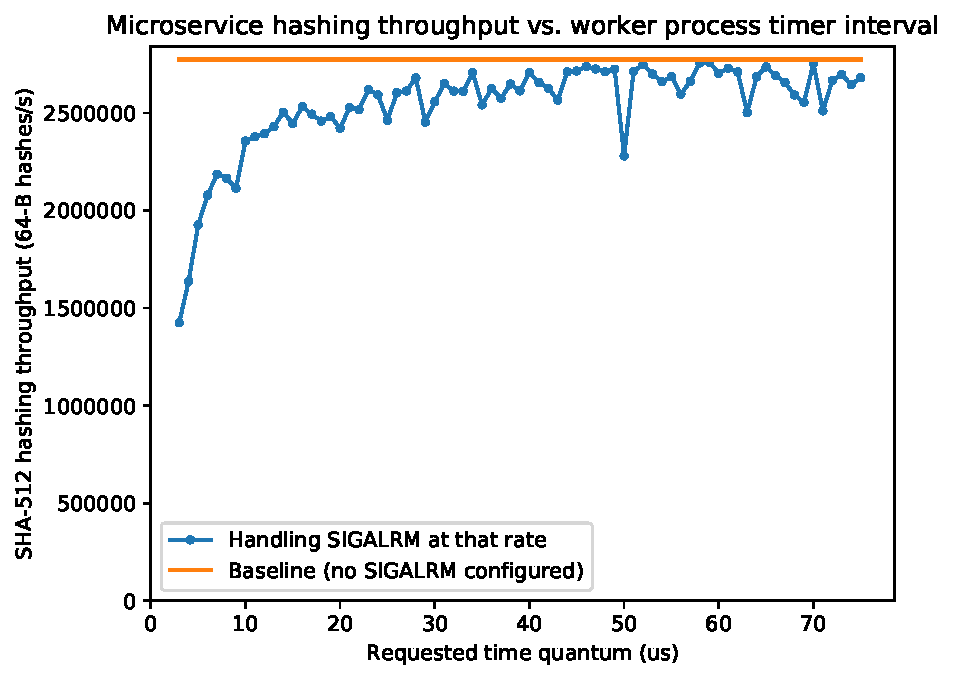
\includegraphics[width=\columnwidth]{figs/2018-02-02-evaluation_quantum-hasher_throughput-throughput}
\caption{Effect of \texttt{SIGALRM} quantum on hashing tput.}
\label{fig:hashtput}
\end{figure}

\paragraph{How do we clean up a terminated microservice?}
We now discuss our mechanism for aborting and cleaning up after a microservice
exceeds its runtime budget.  POSIX signal handlers receive as an argument a pointer to their
\textit{context}, a snapshot of the process's PCB (process control block) at the
moment before it received the signal.  When the handler returns, the system will
transfer control back to the point described by the context, so a naïve way for our
worker processes to regain control would be to reset its GPRs (general-purpose
registers) to values recorded just before the worker's tight scheduling loop.
This approach, however, would not release the microservice's state or memory
allocations back to the worker.

One of the few heavyweight components of the Rust runtime is panic handling,
reminiscent of C++'s exception handling.  The compiler inserts landing pads into each
function that call the destructors for the variables in its stack frame:\@ if the
program ever panics, the standard library uses these to unwind the stack.  We co-opt
this functionality by having the \texttt{SIGALRM} handler set its context to raise an
explicit panic in a fake stack frame just above the real top of the stack.

Section~\ref{sec:future} discusses the limitations and security ramifications of
this approach.
